\documentclass[12pt,a4paper]{article}

% Encodage et langue
\usepackage[utf8]{inputenc}
\usepackage[T1]{fontenc}

% Packages mathématiques et typographiques
\usepackage{amsmath,amssymb}

% Packages requis par kableExtra (tableaux améliorés)
\usepackage{booktabs}
\usepackage{longtable}
\usepackage{array}
\usepackage{multirow}
\usepackage{xcolor}
\usepackage{colortbl}
\usepackage{float}

% Graphiques, mise en page, légendes
\usepackage{graphicx}
\usepackage{setspace}
\usepackage{geometry}
\geometry{margin=2.5cm}
\onehalfspacing
\usepackage{caption}

\title{\textbf{Analyse Exploratoire d'un Corpus Poétique \\
		Étude de la Variable \emph{Anticipation}}}
\author{Étudiant.e \\
	\small{STT-7335 Méthodes d'analyse de données}}
\date{\today}

\begin{document}
	\maketitle
	\tableofcontents
	
	\section{Description du jeu de données}
	Le présent rapport s’appuie sur un ensemble de 3443 vers, chacun annoté par un ensemble
	de variables descriptives concernant l’auteur ou l’autrice ainsi que plusieurs scores émotionnels.
	
	\subsection{Détails des variables du jeu de données}
	Les noms de colonnes dans le fichier source sont listés ci-dessous :
	
	\begin{itemize}
		\item \textbf{poet\_id} : Identifiant unique associé à chaque poète.
		\item \textbf{poet} : Nom du poète ou de la poétesse.
		\item \textbf{suicidal} : Indicateur booléen précisant si l'auteur ou l'autrice
		s'est suicidé(e). La valeur peut être \texttt{TRUE} ou \texttt{FALSE}.
		\item \textbf{period} : Période d'écriture (par exemple, \textit{Early} ou \textit{Modern}).
		\item \textbf{sex} : Sexe de la personne à l'origine du poème (\texttt{Male} ou \texttt{Female}).
		\item \textbf{heterosexual} : Indicateur booléen spécifiant l’orientation sexuelle,
		\texttt{TRUE} pour hétérosexuel(le), \texttt{FALSE} dans les autres cas.
		\item \textbf{date\_of\_birth} : Date de naissance de l'auteur ou de l'autrice.
		\item \textbf{date\_of\_death} : Date de décès de l'auteur ou de l'autrice, si connue.
		\item \textbf{country\_of\_birth} : Pays de naissance.
		\item \textbf{poem\_title} : Titre du poème auquel le vers appartient.
		\item \textbf{n\_words} : Nombre de mots contenus dans le vers.
		\item \textbf{anger} : Score reflétant la présence de la colère dans le vers (valeur numérique).
		\item \textbf{anticipation} : Score reflétant l’anticipation (ou l'attente) véhiculée dans le vers
		(variable réponse principale de cette étude).
		\item \textbf{disgust} : Score reflétant la présence du dégoût dans le vers.
		\item \textbf{fear} : Score reflétant la présence de la peur dans le vers.
		\item \textbf{joy} : Score reflétant la présence de la joie dans le vers.
		\item \textbf{sadness} : Score reflétant la présence de la tristesse dans le vers.
		\item \textbf{surprise} : Score reflétant la présence de la surprise dans le vers.
		\item \textbf{trust} : Score reflétant la confiance véhiculée par le vers.
		\item \textbf{negative} : Score global regroupant des émotions à valence négative.
		\item \textbf{positive} : Score global regroupant des émotions à valence positive.
		\item \textbf{verse} : Position normalisée du vers dans le poème (\texttt{0} : début, \texttt{1} : fin).
	\end{itemize}
	
	Après nettoyage et vérification de la cohérence des données, le corpus final comporte 3443
	vers annotés. Le nombre de données manquantes est faible et n’impacte pas significativement
	les analyses présentées ci-après.
	
	\section{Présentation des variables}
	
	\subsection{Statistiques descriptives}
	Le tableau ci-dessous présente un résumé statistique (minimum, quartiles, médiane, moyenne, maximum)
	des variables numériques, dont \textbf{Anticipation}, \textbf{Colère}, \textbf{Peur}, etc.
	
	\begin{table}
\centering
\caption{\label{tab:tab:summaryStatsFR}Variables numériques : statistiques récapitulatives (en français)}
\centering
\resizebox{\ifdim\width>\linewidth\linewidth\else\width\fi}{!}{
\begin{tabular}[t]{lrrrrrr}
\toprule
Variable & Min & 1er quartile & Médiane & Moyenne & 3e quartile & Max\\
\midrule
\cellcolor{gray!10}{Anticipation} & \cellcolor{gray!10}{0} & \cellcolor{gray!10}{0.00} & \cellcolor{gray!10}{0.0} & \cellcolor{gray!10}{0.15} & \cellcolor{gray!10}{0.00} & \cellcolor{gray!10}{3}\\
Colère & 0 & 0.00 & 0.0 & 0.11 & 0.00 & 4\\
\cellcolor{gray!10}{Confiance} & \cellcolor{gray!10}{0} & \cellcolor{gray!10}{0.00} & \cellcolor{gray!10}{0.0} & \cellcolor{gray!10}{0.13} & \cellcolor{gray!10}{0.00} & \cellcolor{gray!10}{3}\\
Dégoût & 0 & 0.00 & 0.0 & 0.12 & 0.00 & 2\\
\cellcolor{gray!10}{Joie} & \cellcolor{gray!10}{0} & \cellcolor{gray!10}{0.00} & \cellcolor{gray!10}{0.0} & \cellcolor{gray!10}{0.14} & \cellcolor{gray!10}{0.00} & \cellcolor{gray!10}{3}\\
\addlinespace
Nombre de mots & 1 & 5.00 & 7.0 & 6.76 & 8.00 & 40\\
\cellcolor{gray!10}{Négatif} & \cellcolor{gray!10}{0} & \cellcolor{gray!10}{0.00} & \cellcolor{gray!10}{0.0} & \cellcolor{gray!10}{0.33} & \cellcolor{gray!10}{1.00} & \cellcolor{gray!10}{4}\\
Peur & 0 & 0.00 & 0.0 & 0.17 & 0.00 & 4\\
\cellcolor{gray!10}{Positif} & \cellcolor{gray!10}{0} & \cellcolor{gray!10}{0.00} & \cellcolor{gray!10}{0.0} & \cellcolor{gray!10}{0.27} & \cellcolor{gray!10}{0.00} & \cellcolor{gray!10}{4}\\
Surprise & 0 & 0.00 & 0.0 & 0.08 & 0.00 & 2\\
\addlinespace
\cellcolor{gray!10}{Tristesse} & \cellcolor{gray!10}{0} & \cellcolor{gray!10}{0.00} & \cellcolor{gray!10}{0.0} & \cellcolor{gray!10}{0.19} & \cellcolor{gray!10}{0.00} & \cellcolor{gray!10}{3}\\
Vers & 0 & 0.24 & 0.5 & 0.49 & 0.74 & 1\\
\bottomrule
\end{tabular}}
\end{table}
	
	\subsection{Distribution de la variable Anticipation}
	La Figure~\ref{fig:hist_anticipation} montre l'histogramme de la variable \textbf{Anticipation}.
	On constate une forte concentration à 0 et quelques valeurs plus élevées, quoique
	peu fréquentes dans le corpus.
	
	\begin{figure}[H]
		\centering
		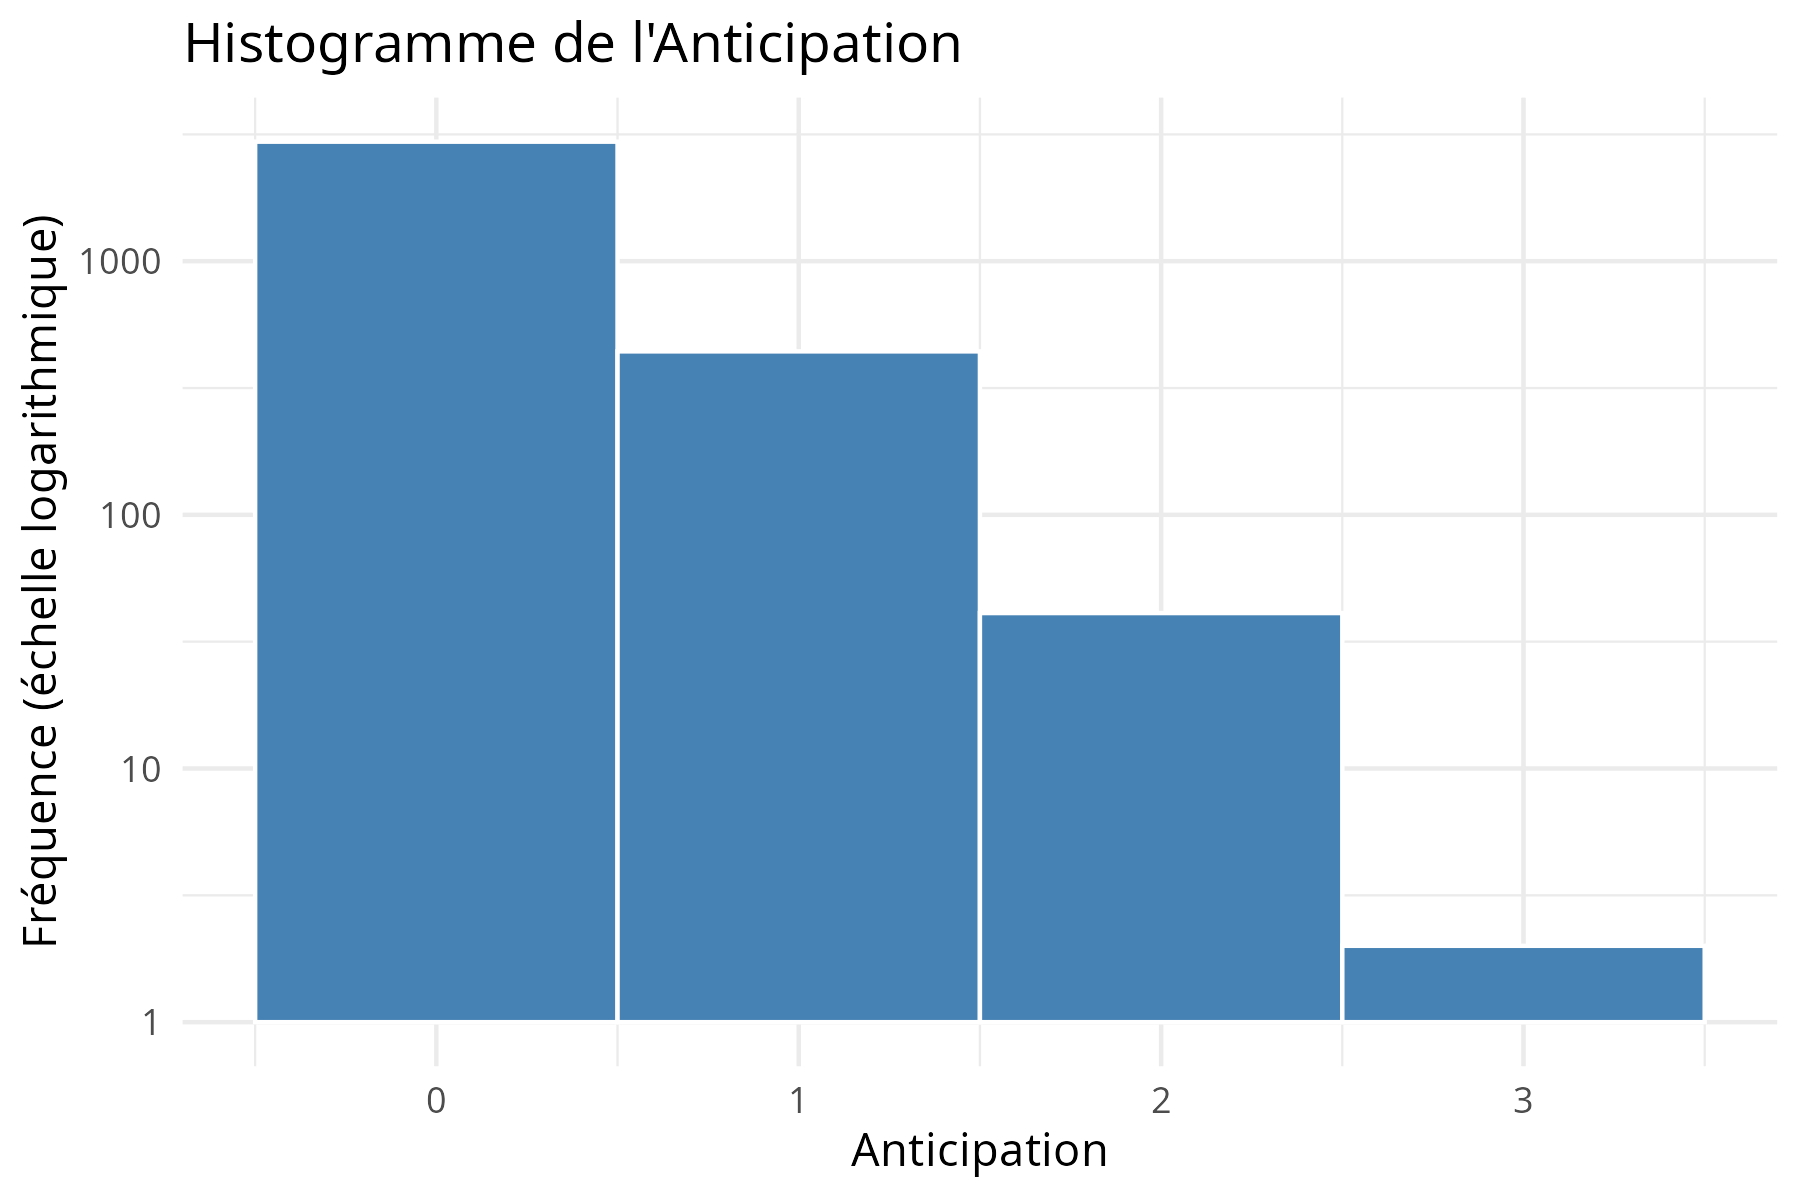
\includegraphics[width=0.6\textwidth]{figures/hist_anticipation.png}
		\caption{Histogramme de la variable \textbf{Anticipation}}
		\label{fig:hist_anticipation}
	\end{figure}
	
	\subsection{Corrélations avec les autres variables émotionnelles}
	Les Figures~\ref{fig:cor_ggcorrplot} et \ref{fig:cor_heatmap} illustrent les
	corrélations entre \textbf{Colère}, \textbf{Anticipation}, \textbf{Dégoût}, \textbf{Peur},
	\textbf{Joie}, \textbf{Tristesse}, \textbf{Surprise}, \textbf{Confiance}, \textbf{Négatif}
	et \textbf{Positif}.
	
	
	\begin{figure}[H]
		\centering
		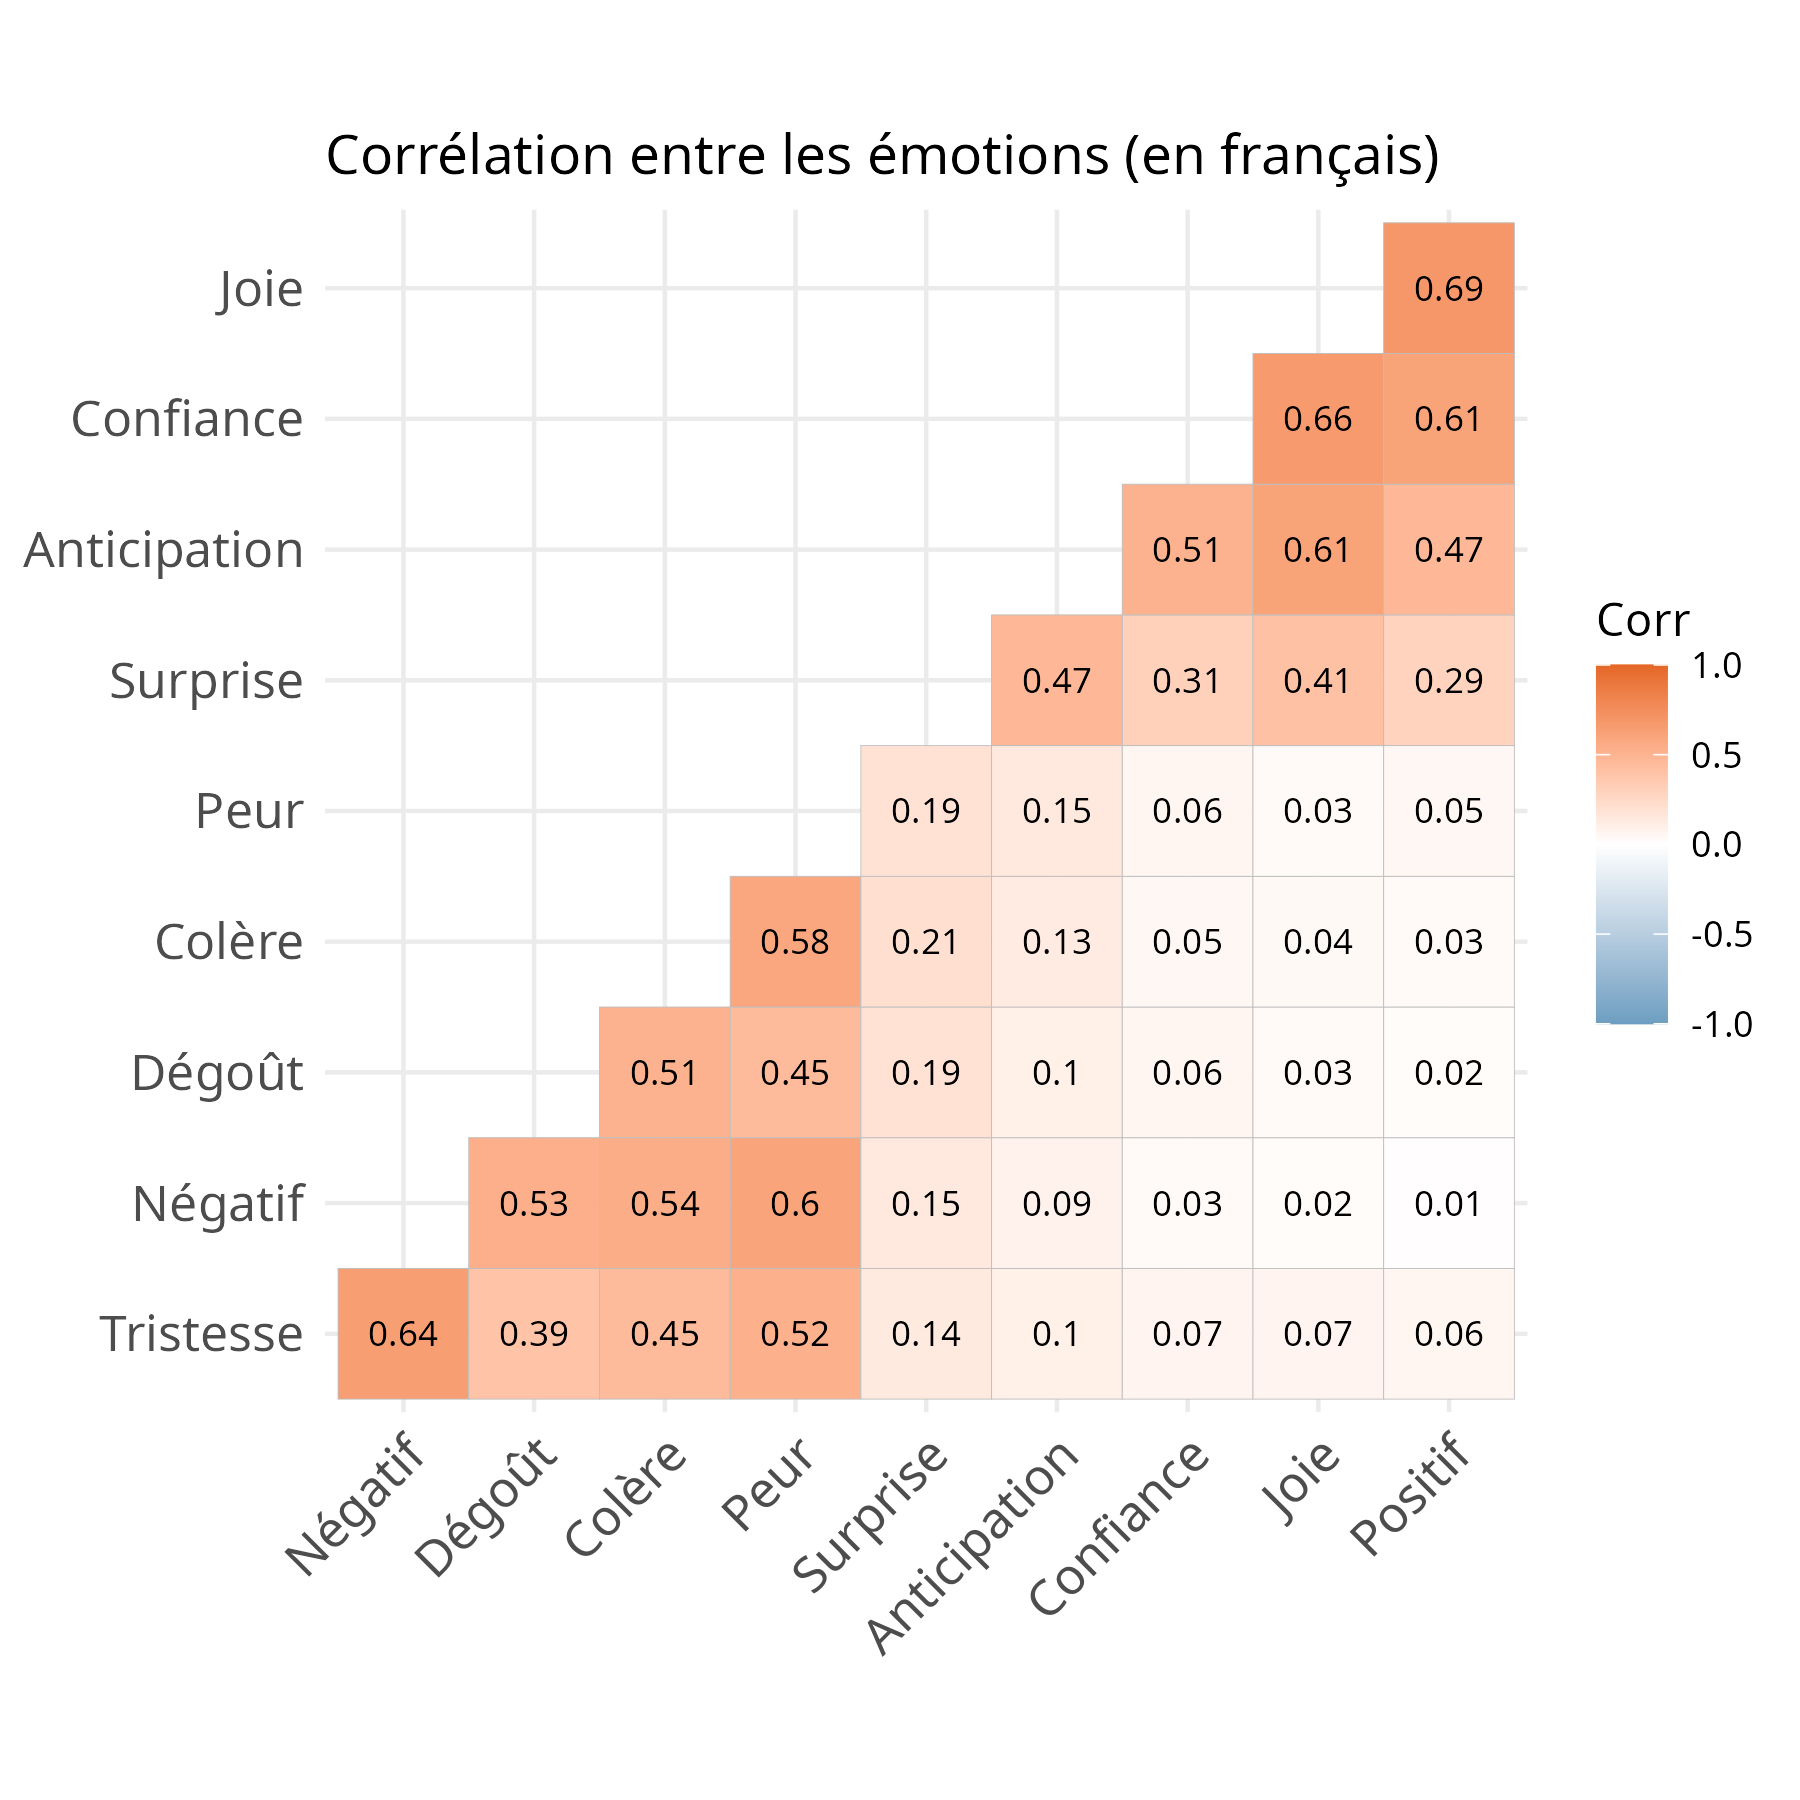
\includegraphics[width=0.65\textwidth]{figures/correlation_ggcorrplot.png}
		\caption{Matrice de corrélation (méthode \texttt{ggcorrplot})}
		\label{fig:cor_ggcorrplot}
	\end{figure}
	
	Cette première représentation indique la valeur des coefficients de corrélation,
	avec un réordonnancement par clustering hiérarchique.
	
	
	\begin{figure}[H]
		\centering
		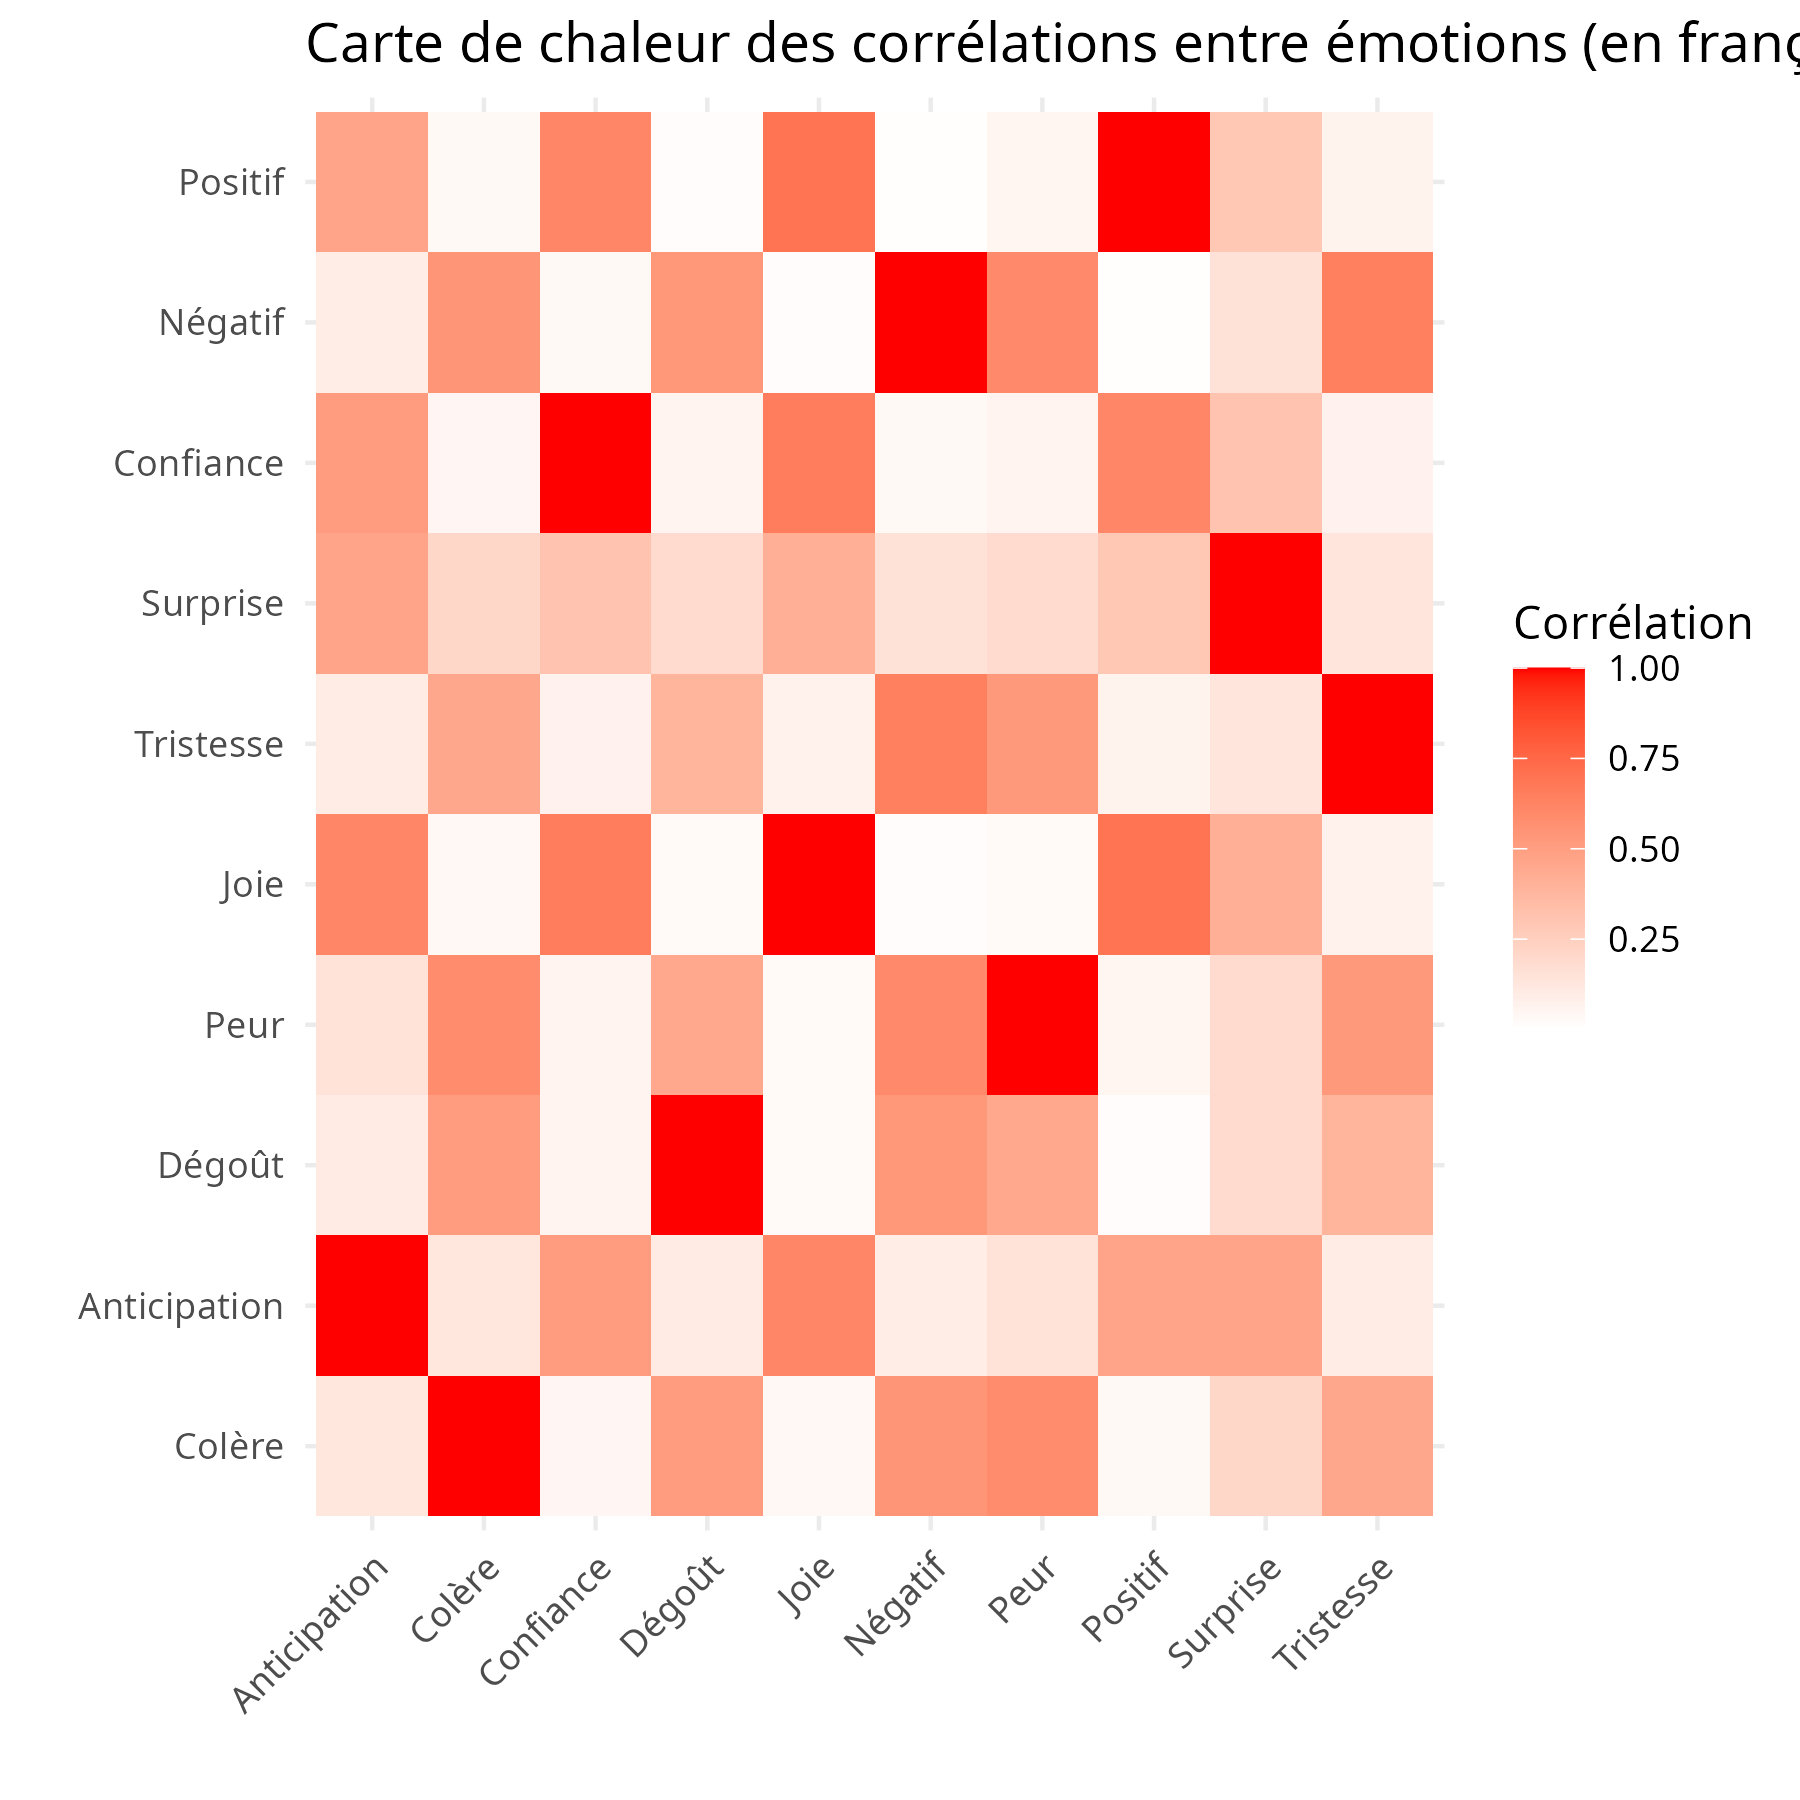
\includegraphics[width=0.65\textwidth]{figures/correlation_heatmap.png}
		\caption{Carte de chaleur de la corrélation entre les émotions}
		\label{fig:cor_heatmap}
	\end{figure}
	
	Cette carte permet de repérer facilement les relations positives et négatives
	entre les différentes émotions. Le bleu reflète des corrélations négatives,
	le rouge des corrélations positives, et le blanc une corrélation nulle.
	
	\section{Analyse avec réduction de la dimension}
	
	\subsection{ACP et éboulis des valeurs propres}
	Afin de mieux cerner la structure multidimensionnelle de ces variables
	émotionnelles, nous appliquons une analyse en composantes principales (ACP).
	La Figure~\ref{fig:pca_scree} présente l’éboulis des valeurs propres, qui illustre
	la part de variance expliquée par chaque axe principal.
	
	\begin{figure}[H]
		\centering
		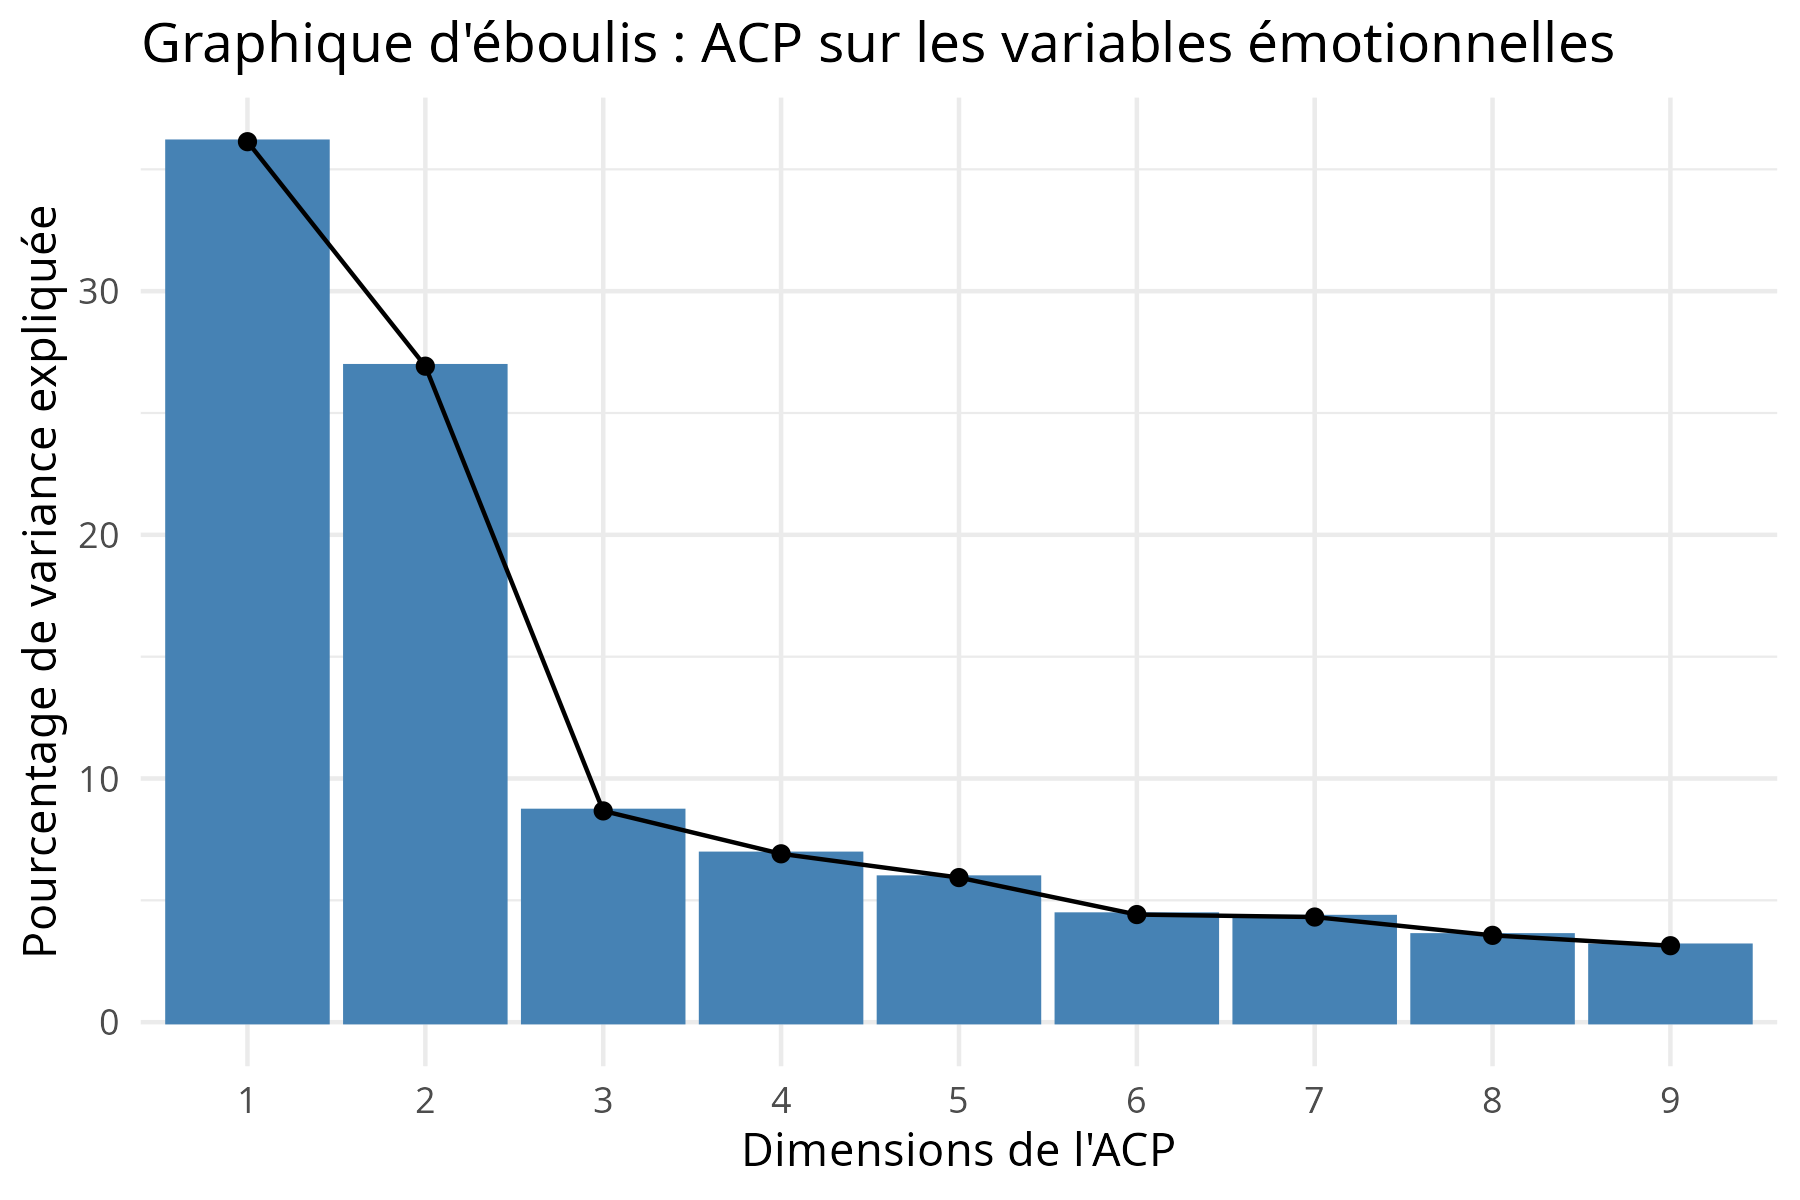
\includegraphics[width=0.65\textwidth]{figures_PCA/pca_screeplot.png}
		\caption{Éboulis (Scree Plot) des composantes principales}
		\label{fig:pca_scree}
	\end{figure}
	
	\subsection{Biplot de l’ACP}
	La Figure~\ref{fig:pca_biplot} montre un biplot où les axes principaux sont
	utilisés pour projeter à la fois les variables (flèches) et les observations
	(points). Les observations sont colorées en fonction de \textbf{Anticipation} afin
	de situer cette variable dans l’espace factoriel.
	
	\begin{figure}[H]
		\centering
		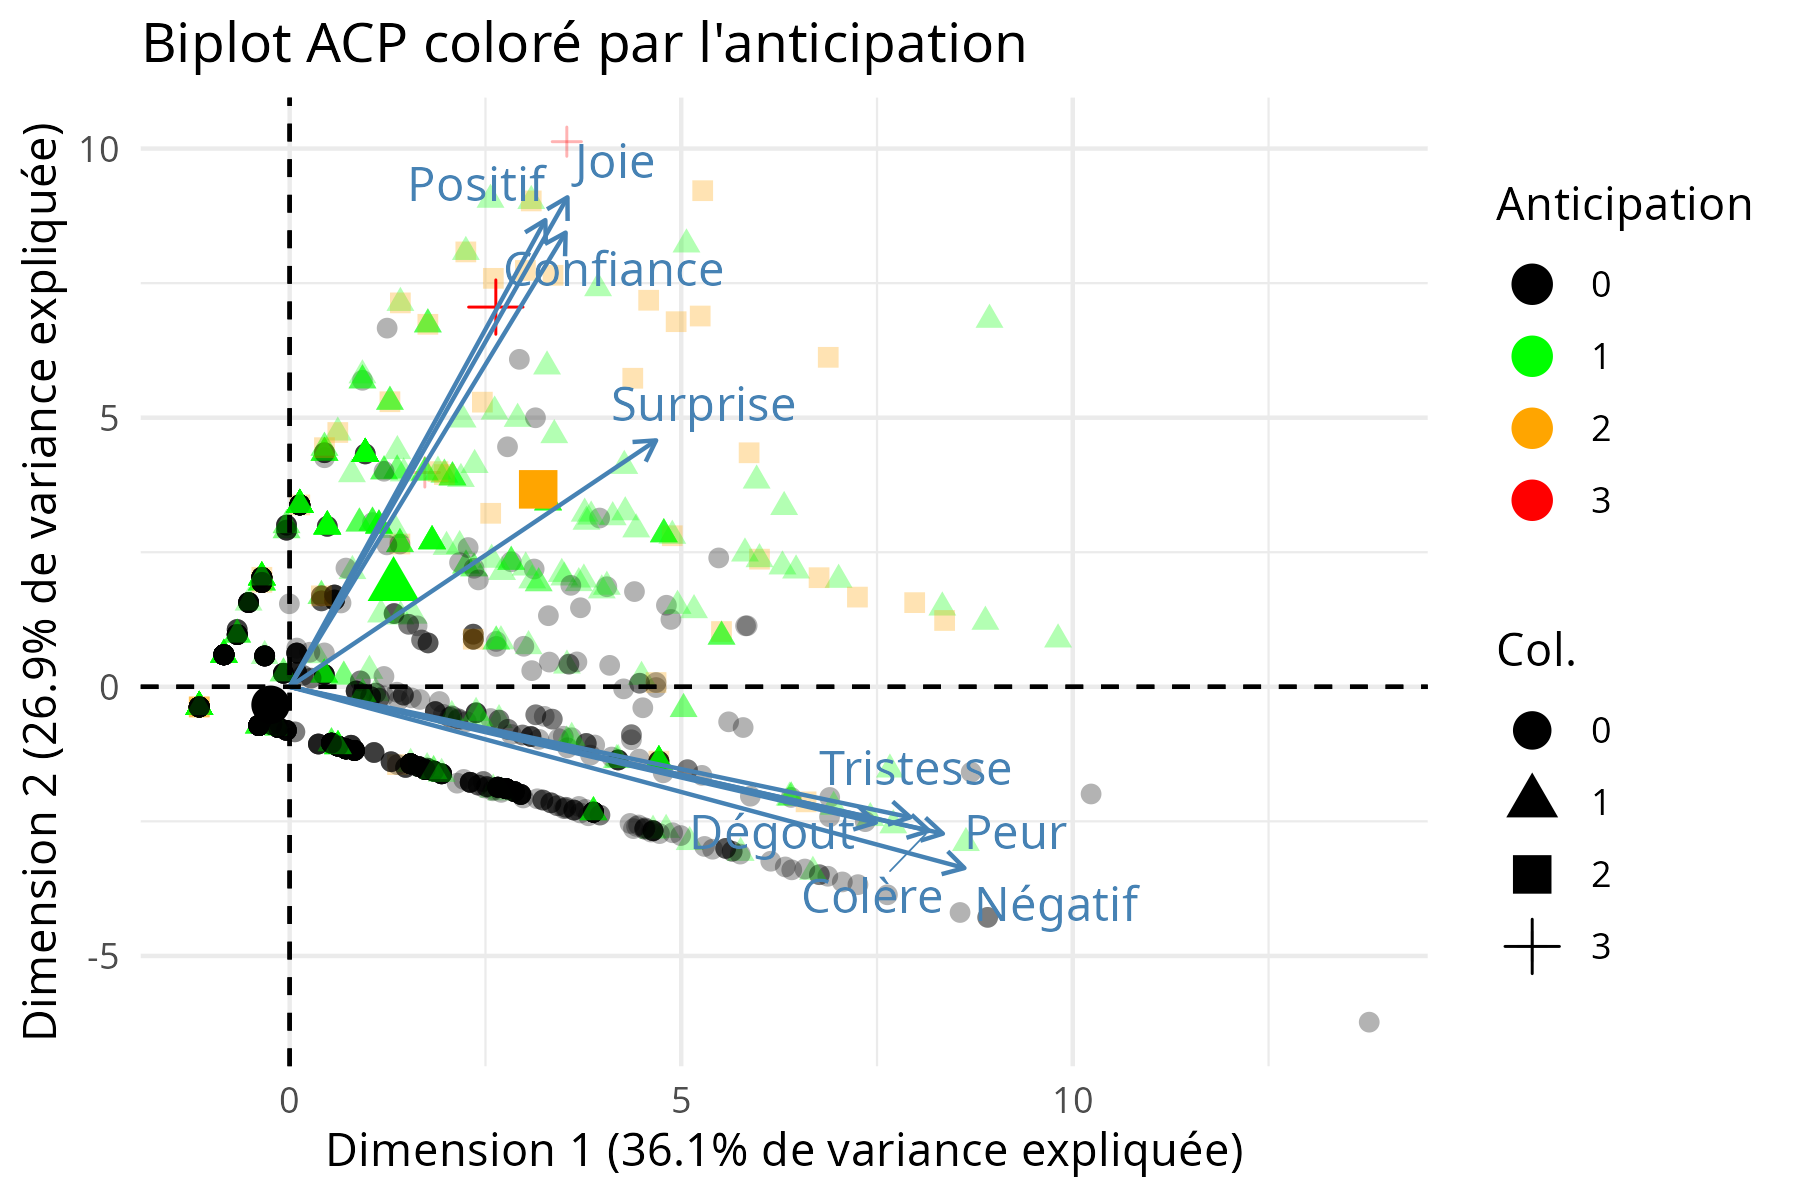
\includegraphics[width=0.75\textwidth]{figures_PCA/pca_biplot_anticipation.png}
		\caption{Biplot de l’ACP, coloré selon la variable Anticipation}
		\label{fig:pca_biplot}
	\end{figure}
	
	On observe que \textbf{Colère}, \textbf{Peur} et \textbf{Négatif} s’opposent
	fortement à \textbf{Joie}, \textbf{Confiance} et \textbf{Positif}. La variable
	\textbf{Anticipation} se retrouve plutôt du côté des émotions positives.
	
	\subsection{Conclusion et perspectives}
	\begin{itemize}
		\item L'analyse révèle une distribution faiblement étalée de la plupart
		des scores émotionnels, \textbf{Anticipation} comprise.
		\item Les corrélations confirment la présence de deux grands ensembles :
		\textbf{Colère}, \textbf{Peur}, \textbf{Dégoût}, \textbf{Négatif} 
		face à \textbf{Joie}, \textbf{Confiance}, \textbf{Positif}, où \textbf{Anticipation}
		semble s'associer davantage à ces dernières.
		\item L’ACP confirme cette dichotomie et met en évidence une forte
		opposition sur le premier axe. Les deux premiers axes expliquent
		la majorité de la variance, ce qui facilite l’interprétation graphique.
	\end{itemize}
	
	Les travaux futurs pourraient inclure un modèle prédictif approfondi
	de la variable \textbf{Anticipation}, en intégrant davantage de
	caractéristiques (par exemple des indicateurs biographiques plus détaillés
	ou des mesures stylistiques). Il serait également intéressant d’évaluer
	d’autres méthodes de réduction de dimension, comme \texttt{t-SNE} ou
	\texttt{MDS}, afin de comparer leurs performances et d’explorer
	d’éventuelles structures non linéaires dans les données.
	
\end{document}
